\chapter{Week 1}

\section{Part 1}
The purpose of the lines that have been commented out in the appendix 1 is to
setup the projection of the camera. This defines a mapping between world space
and view space. By default - when these lines are commented out - this mapping
is defined by an identity matrix, which means that the viewer sees object located
within the $[0,1][0,1]$ intervals with respect to x an y coordinates.

gluOrtho2d as used below defines a scale and a translation so that the viewer sees object
located within $[-10,10][-10,10]$    

glMatrixMode is a primitive that selects the current matrix, so that OpenGL matrix
operations carried after are operated on the one selected (projection or modelview)

\begin{verbatim}
//glMatrixMode (GL_PROJECTION);
//glLoadIdentity ();
//gluOrtho2D (-10., 10., -10., 10.);
//glMatrixMode (GL_MODELVIEW);
\end{verbatim}

\section{Part 2}

Here are the lines modified as requested in the assignment
\begin{verbatim}
 glLoadIdentity ();
glLoadIdentity ();
	glTranslated(1.5,0,0);
	glRotated(45, 0, 0, 1);
	glTranslated(-1.5,0,0);
    glColor3f(1.0,1.0,0.0);
    glBegin (GL_POLYGON);
		glVertex2fv (V[0]);
		glVertex2fv (V[1]);
		glVertex2fv (V[2]);
		glVertex2fv (V[3]);
	glEnd ();

	glLoadIdentity();
	glTranslated(6,7,0);
	glBegin(GL_TRIANGLES);
		glColor3f (1.0, 0.0, 0.0);
		glVertex2f(2.0, 2.0);
		glColor3f (0.0, 1.0, 0.0);
		glVertex2f(5.0, 2.0);
		glColor3f (0.0, 0.0, 1.0);
		glVertex2f(3.5,5);
	glEnd();
glEnd();
\end{verbatim}

This give the following result:

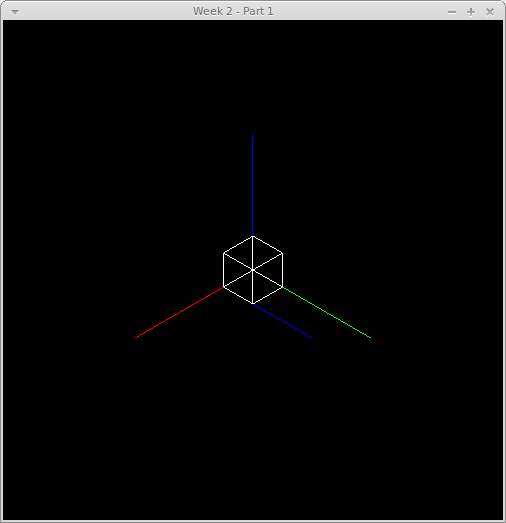
\includegraphics[!h]{Week1/Part1.png}



\section{Part 3}


\section{Part 4}


\section{Part 5}
